
% --- SLIDE 2: THE FORMAL PICTURE ---
\begin{frame}{Drift, Formally}

    \begin{block}{The model learned a joint distribution}
        Training gave you $P_{\text{train}}(X, Y) = P(X)\,P(Y \mid X)$. Deployment assumes
        $P_{\text{serve}} = P_{\text{train}}$. Drift is any way that assumption fails.
    \end{block}

    \vspace{0.12em}
    \centering
    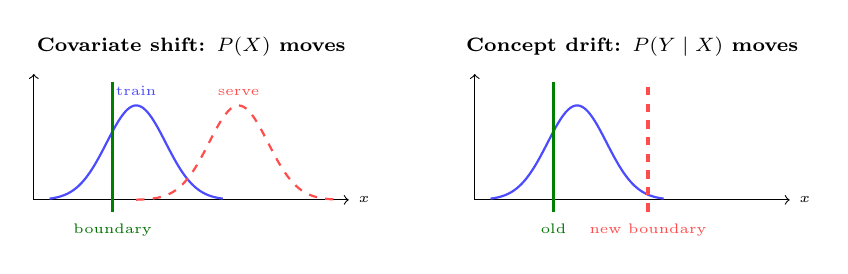
\begin{tikzpicture}[font=\scriptsize]
        % Panel 1: covariate shift -- P(X) moves, the rule does not
        \begin{scope}[shift={(0,0)}]
            \node[font=\scriptsize\bfseries, anchor=south] at (2.0,1.7) {Covariate shift: $P(X)$ moves};
            \draw[->] (0,0) -- (4.0,0) node[right, font=\tiny] {$x$};
            \draw[->] (0,0) -- (0,1.6);
            \draw[blue!70, thick, smooth, domain=0.2:2.4, samples=40]
                plot (\x, {1.2*exp(-(\x-1.3)^2/0.28)});
            \draw[red!70, thick, dashed, smooth, domain=1.3:3.9, samples=40]
                plot (\x, {1.2*exp(-(\x-2.6)^2/0.28)});
            \draw[green!50!black, very thick] (1.0,-0.15) -- (1.0,1.5);
            \node[green!45!black, font=\tiny, anchor=north] at (1.0,-0.18) {boundary};
            \node[blue!70, font=\tiny, anchor=south] at (1.3,1.2) {train};
            \node[red!70, font=\tiny, anchor=south] at (2.6,1.2) {serve};
        \end{scope}
        % Panel 2: concept drift -- P(Y|X) moves, the inputs do not
        \begin{scope}[shift={(5.6,0)}]
            \node[font=\scriptsize\bfseries, anchor=south] at (2.0,1.7) {Concept drift: $P(Y\mid X)$ moves};
            \draw[->] (0,0) -- (4.0,0) node[right, font=\tiny] {$x$};
            \draw[->] (0,0) -- (0,1.6);
            \draw[blue!70, thick, smooth, domain=0.2:2.4, samples=40]
                plot (\x, {1.2*exp(-(\x-1.3)^2/0.28)});
            \draw[green!50!black, very thick] (1.0,-0.15) -- (1.0,1.5);
            \draw[red!70, very thick, dashed] (2.2,-0.15) -- (2.2,1.5);
            \node[green!45!black, font=\tiny, anchor=north] at (1.0,-0.18) {old};
            \node[red!70, font=\tiny, anchor=north] at (2.2,-0.18) {new boundary};
        \end{scope}
    \end{tikzpicture}

    \vspace{0.18em}
    \begin{itemize}
        \scriptsize
        \item \textbf{Left:} the inputs moved but the rule is unchanged. Your model may still be right ---
              it is just being asked questions it was not trained on.
        \item \textbf{Right:} the inputs look identical and the \emph{answer} changed. Nothing in the input
              distribution will tell you. Only labels will.
        \item \textbf{This is why input monitoring alone is not enough} --- and why it is still worth having,
              because it is the only signal available immediately.
    \end{itemize}

\end{frame}
